% Created 2023-05-16 Tue 15:20
% Intended LaTeX compiler: pdflatex
\documentclass[11pt]{article}
\usepackage[utf8]{inputenc}
\usepackage[T1]{fontenc}
\usepackage{graphicx}
\usepackage{longtable}
\usepackage{wrapfig}
\usepackage{rotating}
\usepackage[normalem]{ulem}
\usepackage{amsmath}
\usepackage{amssymb}
\usepackage{capt-of}
\usepackage{hyperref}
\usepackage{tcolorbox}
\usepackage{minted}
\usepackage[margin=1in]{geometry}
\usepackage{xcolor}
\author{Nidish Narayanaa Balaji}
\date{\today}
\title{WaveVib - An OCTAVE/MATLAB Toolbox for Wave-Based Modeling of Nonlinear Jointed Structures}
\hypersetup{
 pdfauthor={Nidish Narayanaa Balaji},
 pdftitle={WaveVib - An OCTAVE/MATLAB Toolbox for Wave-Based Modeling of Nonlinear Jointed Structures},
 pdfkeywords={},
 pdfsubject={},
 pdfcreator={Emacs 29.0.90 (Org mode 9.6.3)}, 
 pdflang={English}}
\makeatletter
\newcommand{\citeprocitem}[2]{\hyper@linkstart{cite}{citeproc_bib_item_#1}#2\hyper@linkend}
\makeatother

\usepackage[notquote]{hanging}
\begin{document}

\maketitle
\tableofcontents


\section{Introduction}
\label{sec:org50d2792}
WaveVib is intended to be a set of OCTAVE/MATLAB routines that can be used to study wave-based linear and nonlinear structures. The main advantage with using this approach comes from the fact that the linear portions of the problem are represented without any approximation (unlike weighted residual or variational approaches). The interface supports both periodic as well as quasi-periodic steady state response regimes. Immediate use cases include jointed beams, trusses, frame structures, fluid-filled columns, rotordynamics, etc.

A good starting place for the new user to the Wave-Based Modeling (WBM) framework \&/or this package are the papers \citeprocitem{1}{[1]}, \citeprocitem{2}{[2]}, upon which most of the rudiments of this package are based.
\subsection{The different folders in the repository}
\label{sec:org0db3823}
\begin{enumerate}
\item \href{../../DEVEL\_PER/}{DEVEL\_PER} [Obsolete]
Contains development scripts used for development of the periodic response routines \& examples.
\item \href{../../DEVEL\_QPER/}{DEVEL\_QPER}
Contains development scripts used for development of the quasi-periodic response routines \& examples.
\item \href{../../EXAMPLES/}{EXAMPLES}
Contains examples with most of the core functionality
\item \href{../../REPS/}{REPS}
Contains miscellaneous reports (under REPn folders) and this main documentation (under the \href{../../REPS/DOCS/}{DOCS} folder)
\item \href{../../ROUTINES/}{ROUTINES}
Contains the core routines of the package.
\end{enumerate}
\section{Programming Interface}
\label{sec:orgad9ca28}
Coming soon\ldots{}
\section{\href{../../EXAMPLES/}{Examples}}
\label{sec:org152067a}
\subsection{\href{../../EXAMPLES/a\_singlebar.m}{Single Bar}}
\label{sec:orgff2da90}
Coming soon\ldots{}
\subsection{\href{../../EXAMPLES/b\_linjointedbars.m}{Linear-Jointed Bars}}
\label{sec:org71e0407}
Coming soon\ldots{}
\subsection{\href{../../EXAMPLES/c\_nljointedbars.m}{Nonlinear-Jointed Bars}}
\label{sec:orgedeed44}
Coming soon\ldots{}
\subsection{\href{../../EXAMPLES/d\_nljointedEBbeams.m}{Nonlinear-Jointed Euler-Bernoulli Beams}}
\label{sec:orgeaca2f1}
Coming soon\ldots{}
\subsection{\href{../../EXAMPLES/e\_nlimpactclbeams.m}{Impacting Cantilever Beams}}
\label{sec:org4724e61}
This is an example from \citeprocitem{3}{[3]}, where the dynamics of an impacting cantilever beam setup is investigated. The technical interest in this example is motivated from the broader are of vibro-impact dynamics\citeprocitem{4}{[4]}, wherein the advantages of the wave based approach are expected to be particularly relevant (due to the avoidance of spatial discretization).

A schematic of the setup is shown below in fig. \ref{fig:org6298ff3} and the material properties used for this example are presented in tab. \ref{tab:org795eda2}.
\begin{figure}[htbp]
\centering
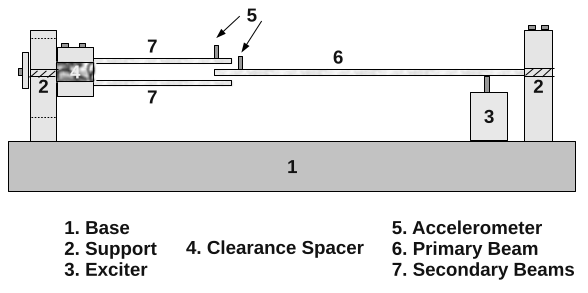
\includegraphics[width=.9\linewidth]{./FIGS/iclbeamsetup.png}
\caption{\label{fig:org6298ff3}Schematic of the impacting cantilever beam setup \citeprocitem{3}{[3]}}
\end{figure}
\begin{table}[htbp]
\caption{\label{tab:org795eda2}Material Properties assumed for the example in \url{../../EXAMPLES/e\_nlimpactclbeams.m}}
\centering
\begin{tabular}{rrllllrr}
Young's Modulus (GPa) & Density (kg/m\textsuperscript{3}) & Section (mm\textsuperscript{2}) & Lengths (mm) & Excitation Point (mm) & Rayleigh damping (\(\alpha\), \(\beta\)) & Contact Gap (mm) & Contact Stiffness (N/m)\\[0pt]
\hline
210 & 7680 & 3 \texttimes{} 40 & 560, 445 & 560/6 & (0.80, 1.1\texttimes{} 10\textsuperscript{-4}) & 2.5 & 110\\[0pt]
\end{tabular}
\end{table}

\subsection{Code Overview}
\label{sec:org1954e0e}
The most important part of the code are from line 16 to line 107. The complete code is explained below in different blocks.
\definecolor{osbe-bg}{HTML}{e5f5e5}\colorlet{osbe-fg}{green}\begin{quote}
                              \begin{tcolorbox}[colback=osbe-bg,colframe=osbe-fg,title={Declare Properties},sharp corners,boxrule=0.4pt]
Here we just assign variables to the properties that will be useful for declaring properties.
\begin{verbatim}
 1  addpath('../ROUTINES/SOLVERS/')
 2  addpath('../ROUTINES/WBM/')
 3  
 4  %% Setup Model
 5  Ey = 2.1e11;
 6  rho = 7680;
 7  thk = 3e-3;   % Thickness 1
 8  wid  = 40e-3;  % Width
 9  Ar = thk*wid;  % Area
10  Iy = thk^3*wid/12;  % 2nd moment of area
11  L1  = 560e-3;  % Primary beam length
12  xF1 = L1/6;    % Excitation Location (on primary beam)
13  L2 = 445e-3;  % Secondary beam length (each)
14  al = 0.80;    % 0.80, 1.80
15  bt = 1.1e-4;  % 1.1e-4, 2.475e-4
16  % Joint parameters
17  knl = 220/2;      % 220,      880,    (242, 484, 880, 1210)
18  gap = 2.5e-3;   % 2.5e-3,   0.35,   0.35
\end{verbatim}


               \end{tcolorbox}
\end{quote}
\definecolor{osbe-bg}{HTML}{e5f5e5}\colorlet{osbe-fg}{green}\begin{quote}
                              \begin{tcolorbox}[colback=osbe-bg,colframe=osbe-fg,title={Declare Dispersion Relationship},sharp corners,boxrule=0.4pt]
Here we declare the dispersion relationship that will be used in the model
\begin{verbatim}
 1  % Declare a library of dispersion relationships (only one here) 
 2  Klib = struct('K', @(w,xi) ((rho*Ar*(w.^2+1j*w*al))./(Ey*Iy*(1-1j*w*bt))).^(0.25) ); 
 3  wcomps = [1 1;  % First component -> exp(  k x )
 4           -1 1;  % Second component-> exp( -k x )
 5           1j 1;  % Third component -> exp( ik x )
 6          -1j 1]; % Fourth component-> exp(-ik x )
 7  
 8  % If multiple dispersion relationships are present in a model, Klib
 9  % must be declared as a vector of structs, and the second column of
10  % wcomps must be used to refer to an appropriate entry in this.
\end{verbatim}
The format is that the 'K' is a function of frequency 'w' and some parameter (could be vector) 'xi'. The array wcomps declares how to use the dispersion relationships from the 'Klib' library structure.


               \end{tcolorbox}
\end{quote}

\section{Desirable Features [2/6]}
\label{sec:org95454df}
\begin{enumerate}
\item{$\square$} 3D frame joint constitutions
\item{$\square$} EPMC Implementation
\item{$\boxtimes$} Joints connecting multiple pieces
\item{$\square$} More detailed examples
\item{$\square$} Stability Implementation
\item{$\boxtimes$} Quasi-Periodic Calculations
\end{enumerate}
\section{References}
\label{sec:org4e3cbf3}
\hypertarget{citeproc_bib_item_1}{[1] N. N. Balaji, M. R. W. Brake, and M. J. Leamy, “Wave-based analysis of jointed elastic bars: Nonlinear periodic response,” \textit{Nonlinear dynamics}, vol. 110, no. 3, pp. 2005–2031, Nov. 2022, doi: \href{https://doi.org/10.1007/s11071-022-07765-0}{10.1007/s11071-022-07765-0}.}

\hypertarget{citeproc_bib_item_2}{[2] N. N. Balaji, M. R. W. Brake, and M. J. Leamy, “Wave-based analysis of jointed elastic bars: Stability of nonlinear solutions,” \textit{Nonlinear dynamics}, vol. 111, no. 3, pp. 1971–1986, Feb. 2023, doi: \href{https://doi.org/10.1007/s11071-022-07969-4}{10.1007/s11071-022-07969-4}.}

\hypertarget{citeproc_bib_item_3}{[3] I. R. Praveen Krishna and C. Padmanabhan, “Experimental and numerical investigations of impacting cantilever beams part 1: First mode response,” \textit{Nonlinear dynamics}, vol. 67, no. 3, pp. 1985–2000, Feb. 2012, doi: \href{https://doi.org/10.1007/s11071-011-0123-2}{10.1007/s11071-011-0123-2}.}

\hypertarget{citeproc_bib_item_4}{[4] E. Emaci, T. A. Nayfeh, and A. F. Vakakis, “Numerical and Experimental Study of Nonlinear Localization in a Flexible Structure with Vibro-Impacts,” \textit{Zamm - journal of applied mathematics and mechanics / zeitschrift für angewandte mathematik und mechanik}, vol. 77, no. 7, pp. 527–541, 1997, doi: \href{https://doi.org/10.1002/zamm.19970770712}{10.1002/zamm.19970770712}.}\bigskip
\end{document}